\documentclass[tikz]{standalone}

\usepackage{pgfplots}
\pgfplotsset{compat=1.9}
\usepackage[swedish]{babel}	
\usepackage[utf8]{inputenc}	

\begin{document}

% This file was created by matplotlib2tikz v0.7.4.
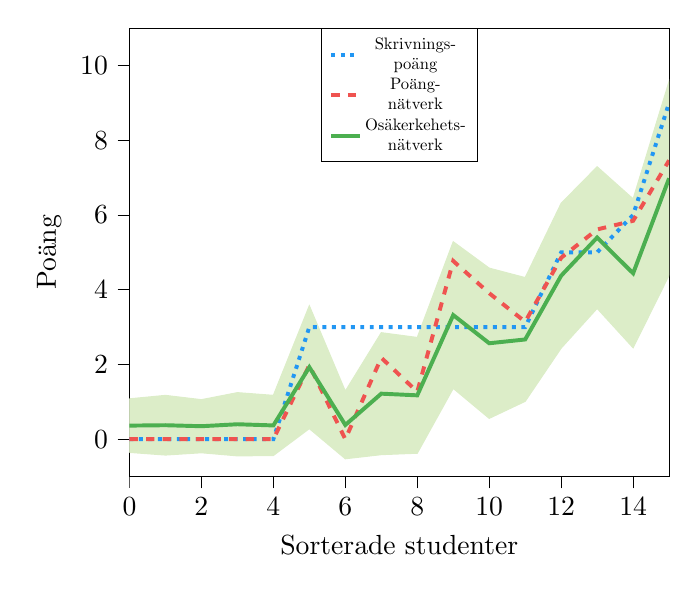
\begin{tikzpicture}

\definecolor{klight_green_100}{RGB}{220, 237, 200}
\definecolor{klight_green_200}{RGB}{197, 225, 165}
\definecolor{klight_green_300}{RGB}{174, 213, 129}
\definecolor{klight_green_400}{RGB}{156, 204, 101}
\definecolor{klight_green_500}{RGB}{139, 195, 74}
\definecolor{kred_100}{RGB}{255, 205, 210}
\definecolor{kred_400}{RGB}{239, 83, 80}
\definecolor{kyellow_400}{RGB}{255, 238, 88}
\definecolor{kgreen_300}{RGB}{129, 199, 132}
\definecolor{kgreen_500}{RGB}{76, 175, 80}
\definecolor{kblue_500}{RGB}{33, 150, 243}
\definecolor{kgrey}{RGB}{222,222,222}
\definecolor{korange}{RGB}{255, 152, 0}  % orange 500

\begin{axis}[
tick align=outside,
tick pos=left,
x grid style={white!69.01960784313725!black},
xlabel={Sorterade studenter},
xmin=0, xmax=15,
xtick style={color=black},
y grid style={white!69.01960784313725!black},
ylabel={Poäng},
ymin=-1, ymax=11,
legend style={at={(0.5, 1)},
                nodes={scale=0.6, transform shape},
                cells={align=center},
                anchor=north,legend columns=1},
legend image post style={scale=0.6},
ytick style={color=black}
]
\path [draw=klight_green_100, fill=klight_green_100]
(axis cs:0,1.07967805862427)
--(axis cs:0,-0.353199899196625)
--(axis cs:1,-0.424238920211792)
--(axis cs:2,-0.362722635269165)
--(axis cs:3,-0.44591760635376)
--(axis cs:4,-0.436850726604462)
--(axis cs:5,0.283388495445251)
--(axis cs:6,-0.523749947547913)
--(axis cs:7,-0.413436770439148)
--(axis cs:8,-0.375537514686584)
--(axis cs:9,1.36030554771423)
--(axis cs:10,0.557525873184204)
--(axis cs:11,1.01342415809631)
--(axis cs:12,2.437659740448)
--(axis cs:13,3.50030326843262)
--(axis cs:14,2.44670534133911)
--(axis cs:15,4.38841915130615)
--(axis cs:15,9.57647800445557)
--(axis cs:15,9.57647800445557)
--(axis cs:14,6.43210554122925)
--(axis cs:13,7.29137897491455)
--(axis cs:12,6.31371641159058)
--(axis cs:11,4.32473182678223)
--(axis cs:10,4.57804012298584)
--(axis cs:9,5.28381156921387)
--(axis cs:8,2.72213268280029)
--(axis cs:7,2.85006761550903)
--(axis cs:6,1.28579413890839)
--(axis cs:5,3.5705714225769)
--(axis cs:4,1.17276573181152)
--(axis cs:3,1.24518096446991)
--(axis cs:2,1.05669987201691)
--(axis cs:1,1.17181348800659)
--(axis cs:0,1.07967805862427)
--cycle;

\addplot [thick, kblue_500, line width=0.5mm, dotted]
table {%
0 0
1 0
2 0
3 0
4 0
5 3
6 3
7 3
8 3
9 3
10 3
11 3
12 5
13 5
14 6
15 9
};
\addplot [thick, kred_400, line width=0.5mm, dashed]
table {%
0 0
1 0
2 0
3 0
4 0
5 1.98138785362244
6 0
7 2.17890596389771
8 1.26910936832428
9 4.76968050003052
10 3.90738224983215
11 3.14235401153564
12 4.85654783248901
13 5.61436939239502
14 5.84549903869629
15 7.46231985092163
};
\addplot [thick, kgreen_500, line width=0.5mm]
table {%
0 0.363239109516144
1 0.3737872838974
2 0.346988618373871
3 0.399631679058075
4 0.367957532405853
5 1.92697989940643
6 0.381022095680237
7 1.21831548213959
8 1.1732976436615
9 3.32205867767334
10 2.56778287887573
11 2.66907787322998
12 4.37568807601929
13 5.39584112167358
14 4.43940544128418
15 6.98244857788086
};
\legend{Skrivnings-\\poäng, Poäng-\\nätverk, Osäkerkehets-\\nätverk}
\end{axis}

\end{tikzpicture}

\end{document}